


\chapter{Conditionals and recursion}

The main topic of this chapter is the {\tt if} statement, which
executes different code depending on the state of the program.
But first I want to introduce two new operators: floor division
and modulus.


\section{Floor division and modulus}

The {\bf floor division} operator, \verb"//", divides
two numbers and rounds down to an integer.  For example, suppose the
run time of a movie is 105 minutes.  You might want to know how
long that is in hours.  Conventional division
returns a floating-point number:

\begin{verbatim}
>>> minutes = 105
>>> minutes / 60
1.75
\end{verbatim}

But we don't normally write hours with decimal points.  Floor
division returns the integer number of hours, dropping the
fraction part:

\begin{verbatim}
>>> minutes = 105
>>> hours = minutes // 60
>>> hours
1
\end{verbatim}

To get the remainder, you could subtract off one hour in minutes:

\begin{verbatim}
>>> remainder = minutes - hours * 60
>>> remainder
45
\end{verbatim}

\index{floor division}
\index{floating-point division}
\index{division!floor}
\index{division!floating-point}
\index{modulus operator}
\index{operator!modulus}

An alternative is to use the {\bf modulus operator}, \verb"%", which
divides two numbers and returns the remainder.

\begin{verbatim}
>>> remainder = minutes % 60
>>> remainder
45
\end{verbatim}
%
The modulus operator is more useful than it seems.  For
example, you can check whether one number is divisible by another---if
{\tt x \% y} is zero, then {\tt x} is divisible by {\tt y}.
\index{divisibility}

Also, you can extract the right-most digit
or digits from a number.  For example, {\tt x \% 10} yields the
right-most digit of {\tt x} (in base 10).  Similarly {\tt x \% 100}
yields the last two digits.

If you are using Python 2, division works differently.  The
division operator, \verb"/", performs floor division if both
operands are integers, and floating-point division if either
operand is a {\tt float}.
\index{Python 2}


\section{Boolean expressions}
\index{boolean expression}
\index{expression!boolean}
\index{logical operator}
\index{operator!logical}

A {\bf boolean expression} is an expression that is either true
or false.  The following examples use the
operator {\tt ==}, which compares two operands and produces
{\tt True} if they are equal and {\tt False} otherwise:

\begin{verbatim}
>>> 5 == 5
True
>>> 5 == 6
False
\end{verbatim}
%
{\tt True} and {\tt False} are special
values that belong to the type {\tt bool}; they are not strings:
\index{True special value}
\index{False special value}
\index{special value!True}
\index{special value!False}
\index{bool type}
\index{type!bool}

\begin{verbatim}
>>> type(True)
<class 'bool'>
>>> type(False)
<class 'bool'>
\end{verbatim}
%
The {\tt ==} operator is one of the {\bf relational operators}; the
others are:

\begin{verbatim}
      x != y               # x is not equal to y
      x > y                # x is greater than y
      x < y                # x is less than y
      x >= y               # x is greater than or equal to y
      x <= y               # x is less than or equal to y
\end{verbatim}
%
Although these operations are probably familiar to you, the Python
symbols are different from the mathematical symbols.  A common error
is to use a single equal sign ({\tt =}) instead of a double equal sign
({\tt ==}).  Remember that {\tt =} is an assignment operator and
{\tt ==} is a relational operator.   There is no such thing as
{\tt =<} or {\tt =>}.
\index{relational operator}
\index{operator!relational}


\section {Logical operators}
\index{logical operator}
\index{operator!logical}

There are three {\bf logical operators}: {\tt and}, {\tt
or}, and {\tt not}.  The semantics (meaning) of these operators is
similar to their meaning in English.  For example,
{\tt x > 0 and x < 10} is true only if {\tt x} is greater than 0
{\em and} less than 10.
\index{and operator}
\index{or operator}
\index{not operator}
\index{operator!and}
\index{operator!or}
\index{operator!not}

{\tt n\%2 == 0 or n\%3 == 0} is true if {\em either or both} of the
conditions is true, that is, if the number is divisible by 2 {\em or}
3.

Finally, the {\tt not} operator negates a boolean
expression, so {\tt not (x > y)} is true if {\tt x > y} is false,
that is, if {\tt x} is less than or equal to {\tt y}.

Strictly speaking, the operands of the logical operators should be
boolean expressions, but Python is not very strict.
Any nonzero number is interpreted as {\tt True}:

\begin{verbatim}
>>> 42 and True
True
\end{verbatim}
%
This flexibility can be useful, but there are some subtleties to
it that might be confusing.  You might want to avoid it (unless
you know what you are doing).


\section{Conditional execution}
\label{conditional.execution}

\index{conditional statement}
\index{statement!conditional}
\index{if statement}
\index{statement!if}
\index{conditional execution}
In order to write useful programs, we almost always need the ability
to check conditions and change the behavior of the program
accordingly.  {\bf Conditional statements} give us this ability.  The
simplest form is the {\tt if} statement:

\begin{verbatim}
if x > 0:
    print('x is positive')
\end{verbatim}
%
The boolean expression after {\tt if} is
called the {\bf condition}.  If it is true, the indented
statement runs.  If not, nothing happens.
\index{condition}
\index{compound statement}
\index{statement!compound}

{\tt if} statements have the same structure as function definitions:
a header followed by an indented body.  Statements like this are
called {\bf compound statements}.

There is no limit on the number of statements that can appear in
the body, but there has to be at least one.
Occasionally, it is useful to have a body with no statements (usually
as a place keeper for code you haven't written yet).  In that
case, you can use the {\tt pass} statement, which does nothing.
\index{pass statement}
\index{statement!pass}

\begin{verbatim}
if x < 0:
    pass          # TODO: need to handle negative values!
\end{verbatim}
%

\section{Alternative execution}
\label{alternative.execution}
\index{alternative execution}
\index{else keyword}
\index{keyword!else}

A second form of the {\tt if} statement is ``alternative execution'',
in which there are two possibilities and the condition determines
which one runs.  The syntax looks like this:

\begin{verbatim}
if x % 2 == 0:
    print('x is even')
else:
    print('x is odd')
\end{verbatim}
%
If the remainder when {\tt x} is divided by 2 is 0, then we know that
{\tt x} is even, and the program displays an appropriate message.  If
the condition is false, the second set of statements runs.
Since the condition must be true or false, exactly one of the
alternatives will run.  The alternatives are called {\bf
  branches}, because they are branches in the flow of execution.
\index{branch}



\section{Chained conditionals}
\index{chained conditional}
\index{conditional!chained}

Sometimes there are more than two possibilities and we need more than
two branches.  One way to express a computation like that is a {\bf
chained conditional}:

\begin{verbatim}
if x < y:
    print('x is less than y')
elif x > y:
    print('x is greater than y')
else:
    print('x and y are equal')
\end{verbatim}
%
{\tt elif} is an abbreviation of ``else if''.  Again, exactly one
branch will run.  There is no limit on the number of {\tt
elif} statements.  If there is an {\tt else} clause, it has to be
at the end, but there doesn't have to be one.
\index{elif keyword}
\index{keyword!elif}

\begin{verbatim}
if choice == 'a':
    draw_a()
elif choice == 'b':
    draw_b()
elif choice == 'c':
    draw_c()
\end{verbatim}
%
Each condition is checked in order.  If the first is false,
the next is checked, and so on.  If one of them is
true, the corresponding branch runs and the statement
ends.  Even if more than one condition is true, only the
first true branch runs.


\section{Nested conditionals}
\index{nested conditional}
\index{conditional!nested}

One conditional can also be nested within another.  We could have
written the example in the previous section like this:

\begin{verbatim}
if x == y:
    print('x and y are equal')
else:
    if x < y:
        print('x is less than y')
    else:
        print('x is greater than y')
\end{verbatim}
%
The outer conditional contains two branches.  The
first branch contains a simple statement.  The second branch
contains another {\tt if} statement, which has two branches of its
own.  Those two branches are both simple statements,
although they could have been conditional statements as well.

Although the indentation of the statements makes the structure
apparent, {\bf nested conditionals} become difficult to read very
quickly.  It is a good idea to avoid them when you can.

Logical operators often provide a way to simplify nested conditional
statements.  For example, we can rewrite the following code using a
single conditional:

\begin{verbatim}
if 0 < x:
    if x < 10:
        print('x is a positive single-digit number.')
\end{verbatim}
%
The {\tt print} statement runs only if we make it past both
conditionals, so we can get the same effect with the {\tt and} operator:

\begin{verbatim}
if 0 < x and x < 10:
    print('x is a positive single-digit number.')
\end{verbatim}

For this kind of condition, Python provides a more concise option:

\begin{verbatim}
if 0 < x < 10:
    print('x is a positive single-digit number.')
\end{verbatim}


\section{Recursion}
\label{recursion}
\index{recursion}

It is legal for one function to call another;
it is also legal for a function to call itself.  It may not be obvious
why that is a good thing, but it turns out to be one of the most
magical things a program can do.
For example, look at the following function:

\begin{verbatim}
def countdown(n):
    if n <= 0:
        print('Blastoff!')
    else:
        print(n)
        countdown(n-1)
\end{verbatim}
%
If {\tt n} is 0 or negative, it outputs the word, ``Blastoff!''
Otherwise, it outputs {\tt n} and then calls a function named {\tt
countdown}---itself---passing {\tt n-1} as an argument.

What happens if we call this function like this?

\begin{verbatim}
>>> countdown(3)
\end{verbatim}
%
The execution of {\tt countdown} begins with {\tt n=3}, and since
{\tt n} is greater than 0, it outputs the value 3, and then calls itself...

\begin{quote}
The execution of {\tt countdown} begins with {\tt n=2}, and since
{\tt n} is greater than 0, it outputs the value 2, and then calls itself...

\begin{quote}
The execution of {\tt countdown} begins with {\tt n=1}, and since
{\tt n} is greater than 0, it outputs the value 1, and then calls itself...

\begin{quote}
The execution of {\tt countdown} begins with {\tt n=0}, and since {\tt
n} is not greater than 0, it outputs the word, ``Blastoff!'' and then
returns.
\end{quote}

The {\tt countdown} that got {\tt n=1} returns.
\end{quote}

The {\tt countdown} that got {\tt n=2} returns.
\end{quote}

The {\tt countdown} that got {\tt n=3} returns.

And then you're back in \verb"__main__".  So, the
total output looks like this:

\begin{verbatim}
3
2
1
Blastoff!
\end{verbatim}
%
A function that calls itself is {\bf recursive}; the process of
executing it is called {\bf recursion}.
\index{recursion}
\index{function!recursive}

As another example, we can write a function that prints a
string {\tt n} times.

\begin{verbatim}
def print_n(s, n):
    if n <= 0:
        return
    print(s)
    print_n(s, n-1)
\end{verbatim}
%
If {\tt n <= 0} the {\bf return statement} exits the function.  The
flow of execution immediately returns to the caller, and the remaining
lines of the function don't run.
\index{return statement}
\index{statement!return}

The rest of the function is similar to {\tt countdown}: it displays
{\tt s} and then calls itself to display {\tt s} $n-1$ additional
times.  So the number of lines of output is {\tt 1 + (n - 1)}, which
adds up to {\tt n}.

For simple examples like this, it is probably easier to use a {\tt
for} loop.  But we will see examples later that are hard to write
with a {\tt for} loop and easy to write with recursion, so it is
good to start early.
\index{for loop}
\index{loop!for}


\section{Stack diagrams for recursive functions}
\label{recursive.stack}
\index{stack diagram}
\index{function frame}
\index{frame}

In Section~\ref{stackdiagram}, we used a stack diagram to represent
the state of a program during a function call.  The same kind of
diagram can help interpret a recursive function.

Every time a function gets called, Python creates a
frame to contain the function's local variables and parameters.
For a recursive function, there might be more than one frame on the
stack at the same time.

Figure~\ref{fig.stack2} shows a stack diagram for {\tt countdown} called with
{\tt n = 3}.

\begin{figure}
\centerline
{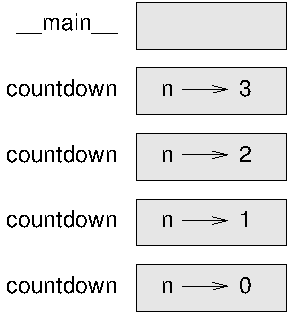
\includegraphics[scale=0.8]{../source/figs/stack2.pdf}}
\caption{Stack diagram.}
\label{fig.stack2}
\end{figure}


As usual, the top of the stack is the frame for \verb"__main__".
It is empty because we did not create any variables in
\verb"__main__" or pass any arguments to it.
\index{base case}
\index{recursion!base case}

The four {\tt countdown} frames have different values for the
parameter {\tt n}.  The bottom of the stack, where {\tt n=0}, is
called the {\bf base case}.  It does not make a recursive call, so
there are no more frames.

As an exercise, draw a stack diagram for \verb"print_n" called with
\verb"s = 'Hello'" and {\tt n=2}.
Then write a function called \verb"do_n" that takes a function
object and a number, {\tt n}, as arguments, and that calls
the given function {\tt n} times.


\section{Infinite recursion}
\index{infinite recursion}
\index{recursion!infinite}
\index{runtime error}
\index{error!runtime}
\index{traceback}

If a recursion never reaches a base case, it goes on making
recursive calls forever, and the program never terminates.  This is
known as {\bf infinite recursion}, and it is generally not
a good idea.  Here is a minimal program with an infinite recursion:

\begin{verbatim}
def recurse():
    recurse()
\end{verbatim}
%
In most programming environments, a program with infinite recursion
does not really run forever.  Python reports an error
message when the maximum recursion depth is reached:
\index{exception!RuntimeError}
\index{RuntimeError}

\begin{verbatim}
  File "<stdin>", line 2, in recurse
  File "<stdin>", line 2, in recurse
  File "<stdin>", line 2, in recurse
                  .
                  .
                  .
  File "<stdin>", line 2, in recurse
RuntimeError: Maximum recursion depth exceeded
\end{verbatim}
%
This traceback is a little bigger than the one we saw in the
previous chapter.  When the error occurs, there are 1000
{\tt recurse} frames on the stack!

If you write encounter an infinite recursion by accident, review
your function to confirm that there is a base case that does not
make a recursive call.  And if there is a base case, check whether
you are guaranteed to reach it.


\section{Keyboard input}
\index{keyboard input}

The programs we have written so far accept no input from the user.
They just do the same thing every time.

Python provides a built-in function called {\tt input} that
stops the program and
waits for the user to type something.  When the user presses {\sf
  Return} or {\sf Enter}, the program resumes and \verb"input"
returns what the user typed as a string.  In Python 2, the same
function is called \verb"raw_input".
\index{Python 2}
\index{input function}
\index{function!input}

\begin{verbatim}
>>> text = input()
What are you waiting for?
>>> text
What are you waiting for?
\end{verbatim}
%
Before getting input from the user, it is a good idea to print a
prompt telling the user what to type.  \verb"input" can take a
prompt as an argument:
\index{prompt}

\begin{verbatim}
>>> name = input('What...is your name?\n')
What...is your name?
Arthur, King of the Britons!
>>> name
Arthur, King of the Britons!
\end{verbatim}
%
The sequence \verb"\n" at the end of the prompt represents a {\bf
  newline}, which is a special character that causes a line break.
That's why the user's input appears below the prompt.  \index{newline}

If you expect the user to type an integer, you can try to convert
the return value to {\tt int}:

\begin{verbatim}
>>> prompt = 'What...is the airspeed velocity of an unladen swallow?\n'
>>> speed = input(prompt)
What...is the airspeed velocity of an unladen swallow?
42
>>> int(speed)
42
\end{verbatim}
%
But if the user types something other than a string of digits,
you get an error:

\begin{verbatim}
>>> speed = input(prompt)
What...is the airspeed velocity of an unladen swallow?
What do you mean, an African or a European swallow?
>>> int(speed)
ValueError: invalid literal for int() with base 10
\end{verbatim}
%
We will see how to handle this kind of error later.
\index{ValueError}
\index{exception!ValueError}


\section{Debugging}
\label{whitespace}
\index{debugging}
\index{traceback}

When a syntax or runtime error occurs, the error message contains
a lot of information, but it can be overwhelming.  The most
useful parts are usually:

\begin{itemize}

\item What kind of error it was, and

\item Where it occurred.

\end{itemize}

Syntax errors are usually easy to find, but there are a few
gotchas.  Whitespace errors can be tricky because spaces and
tabs are invisible and we are used to ignoring them.
\index{whitespace}

\begin{verbatim}
>>> x = 5
>>>  y = 6
  File "<stdin>", line 1
    y = 6
    ^
IndentationError: unexpected indent
\end{verbatim}
%
In this example, the problem is that the second line is indented by
one space.  But the error message points to {\tt y}, which is
misleading.  In general, error messages indicate where the problem was
discovered, but the actual error might be earlier in the code,
sometimes on a previous line.
\index{error!runtime}
\index{runtime error}

The same is true of runtime errors.  Suppose you are trying
to compute a signal-to-noise ratio in decibels.  The formula
is $SNR_{db} = 10 \log_{10} (P_{signal} / P_{noise})$.  In Python,
you might write something like this:

\begin{verbatim}
import math
signal_power = 9
noise_power = 10
ratio = signal_power // noise_power
decibels = 10 * math.log10(ratio)
print(decibels)
\end{verbatim}
%
When you run this program, you get an exception:
%
\index{exception!OverflowError}
\index{OverflowError}

\begin{verbatim}
Traceback (most recent call last):
  File "snr.py", line 5, in ?
    decibels = 10 * math.log10(ratio)
ValueError: math domain error
\end{verbatim}
%
The error message indicates line 5, but there is nothing
wrong with that line.  To find the real error, it might be
useful to print the value of {\tt ratio}, which turns out to
be 0.  The problem is in line 4, which uses floor division
instead of floating-point division.
\index{floor division}
\index{division!floor}

You should take the time to read error messages carefully, but don't
assume that everything they say is correct.


\section{Glossary}

\begin{description}

\item[floor division:] An operator, denoted {\tt //}, that divides two
  numbers and rounds down (toward zero) to an integer.
  \index{floor division}
  \index{division!floor}

\item[modulus operator:]  An operator, denoted with a percent sign
({\tt \%}), that works on integers and returns the remainder when one
number is divided by another.
\index{modulus operator}
\index{operator!modulus}

\item[boolean expression:]  An expression whose value is either
{\tt True} or {\tt False}.
\index{boolean expression}
\index{expression!boolean}

\item[relational operator:] One of the operators that compares
its operands: {\tt ==}, {\tt !=}, {\tt >}, {\tt <}, {\tt >=}, and {\tt <=}.

\item[logical operator:] One of the operators that combines boolean
expressions: {\tt and}, {\tt or}, and {\tt not}.

\item[conditional statement:]  A statement that controls the flow of
execution depending on some condition.
\index{conditional statement}
\index{statement!conditional}

\item[condition:] The boolean expression in a conditional statement
that determines which branch runs.
\index{condition}

\item[compound statement:]  A statement that consists of a header
and a body.  The header ends with a colon (:).  The body is indented
relative to the header.
\index{compound statement}

\item[branch:] One of the alternative sequences of statements in
a conditional statement.
\index{branch}

\item[chained conditional:]  A conditional statement with a series
of alternative branches.
\index{chained conditional}
\index{conditional!chained}

\item[nested conditional:]  A conditional statement that appears
in one of the branches of another conditional statement.
\index{nested conditional}
\index{conditional!nested}

\item[return statement:] A statement that causes a function to
end immediately and return to the caller.

\item[recursion:]  The process of calling the function that is
currently executing.
\index{recursion}

\item[base case:]  A conditional branch in a
recursive function that does not make a recursive call.
\index{base case}

\item[infinite recursion:]  A recursion that doesn't have a
base case, or never reaches it.  Eventually, an infinite recursion
causes a runtime error.
\index{infinite recursion}

\end{description}

\section{Exercises}

\begin{exercise}

The {\tt time} module provides a function, also named {\tt time}, that
returns the current Greenwich Mean Time in ``the epoch'', which is
an arbitrary time used as a reference point.  On UNIX systems, the
epoch is 1 January 1970.

\begin{verbatim}
>>> import time
>>> time.time()
1437746094.5735958
\end{verbatim}

Write a script that reads the current time and converts it to
a time of day in hours, minutes, and seconds, plus the number of
days since the epoch.

\end{exercise}


\begin{exercise}
\index{Fermat's Last Theorem}

Fermat's Last Theorem says that there are no positive integers
$a$, $b$, and $c$ such that

\[ a^n + b^n = c^n \]
%
for any values of $n$ greater than 2.

\begin{enumerate}

\item Write a function named \verb"check_fermat" that takes four
parameters---{\tt a}, {\tt b}, {\tt c} and {\tt n}---and
checks to see if Fermat's theorem holds.  If
$n$ is greater than 2 and

\[a^n + b^n = c^n \]
%
the program should print, ``Holy smokes, Fermat was wrong!''
Otherwise the program should print, ``No, that doesn't work.''

\item Write a function that prompts the user to input values
for {\tt a}, {\tt b}, {\tt c} and {\tt n}, converts them to
integers, and uses \verb"check_fermat" to check whether they
violate Fermat's theorem.

\end{enumerate}

\end{exercise}


\begin{exercise}
\index{triangle}

If you are given three sticks, you may or may not be able to arrange
them in a triangle.  For example, if one of the sticks is 12 inches
long and the other two are one inch long, you will
not be able to get the short sticks to meet in the middle.  For any
three lengths, there is a simple test to see if it is possible to form
a triangle:

\begin{quotation}
If any of the three lengths is greater than the sum of the other
  two, then you cannot form a triangle.  Otherwise, you
  can.  (If the sum of two lengths equals the third, they form
    what is called a ``degenerate'' triangle.)
\end{quotation}

\begin{enumerate}

\item Write a function named \verb"is_triangle" that takes three
  integers as arguments, and that prints either ``Yes'' or ``No'', depending
  on whether you can or cannot form a triangle from sticks with the
  given lengths.

\item Write a function that prompts the user to input three stick
  lengths, converts them to integers, and uses \verb"is_triangle" to
  check whether sticks with the given lengths can form a triangle.

\end{enumerate}

\end{exercise}

\begin{exercise}
What is the output of the following program?
Draw a stack diagram that shows the state of the program
when it prints the result.

\begin{verbatim}
def recurse(n, s):
    if n == 0:
        print(s)
    else:
        recurse(n-1, n+s)

recurse(3, 0)
\end{verbatim}

\begin{enumerate}

\item What would happen if you called this function like this: {\tt
  recurse(-1, 0)}?

\item Write a docstring that explains everything someone would need to
  know in order to use this function (and nothing else).

\end{enumerate}

\end{exercise}


The following exercises use the {\tt turtle} module, described in
Chapter~\ref{turtlechap}:
\index{TurtleWorld}

\begin{exercise}

Read the following function and see if you can figure out
what it does.  Then run it (see the examples in Chapter~\ref{turtlechap}).

\begin{verbatim}
def draw(t, length, n):
    if n == 0:
        return
    angle = 50
    t.fd(length*n)
    t.lt(angle)
    draw(t, length, n-1)
    t.rt(2*angle)
    draw(t, length, n-1)
    t.lt(angle)
    t.bk(length*n)
\end{verbatim}

\end{exercise}


\begin{figure}
\centerline
{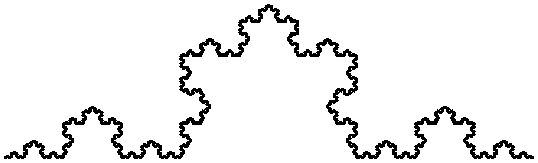
\includegraphics[scale=0.8]{../source/figs/koch.pdf}}
\caption{A Koch curve.}
\label{fig.koch}
\end{figure}

\begin{exercise}
\index{Koch curve}

The Koch curve is a fractal that looks something like
Figure~\ref{fig.koch}.  To draw a Koch curve with length $x$, all you
have to do is

\begin{enumerate}

\item Draw a Koch curve with length $x/3$.

\item Turn left 60 degrees.

\item Draw a Koch curve with length $x/3$.

\item Turn right 120 degrees.

\item Draw a Koch curve with length $x/3$.

\item Turn left 60 degrees.

\item Draw a Koch curve with length $x/3$.

\end{enumerate}

The exception is if $x$ is less than 3: in that case,
you can just draw a straight line with length $x$.

\begin{enumerate}

\item Write a function called {\tt koch} that takes a turtle and
a length as parameters, and that uses the turtle to draw a Koch
curve with the given length.

\item Write a function called {\tt snowflake} that draws three
Koch curves to make the outline of a snowflake.

Solution: \url{http://thinkpython2.com/code/koch.py}.

\item The Koch curve can be generalized in several ways.  See
\url{http://en.wikipedia.org/wiki/Koch_snowflake} for examples and
implement your favorite.

\end{enumerate}
\end{exercise}
